\clearpage

\section{Validation du design} \label{sec:Validation-design}
Dans cette section, nous décrirons la procédure de vérification des caractéristiques du projet ainsi que sa validation.

\subsection{Liste de matériel} \label{ssec:Liste-materiel}
\begin{itemize}
	\item \textbf{P1} : Oscilloscope Tektronix RTB2004 ES.SLO2.05.01.11
	\item \textbf{P2} : Multimètre GwInstek GDM-396 ES.SLO2.00.00.94
	\item Carte Mini-Boite-Noire 1924B
\end{itemize}

\subsection{Consommations}
Dans cette section, nous mesurerons les différentes consommations du système. Cette étape est importante pour caractériser le système et déterminer son autonomie.

\subsubsection{Méthode de mesure}
L'objectif est de basculer entre les différents modes (veille, logging...) de la carte et d'en mesurer la consommation. À cet effet, un ampèremètre a été placé en série avec la batterie, comme illustré à la figure \ref{fig:schema-courant}.

\subsubsection{Schéma de mesure}

\begin{figure}[h]
	\centering
	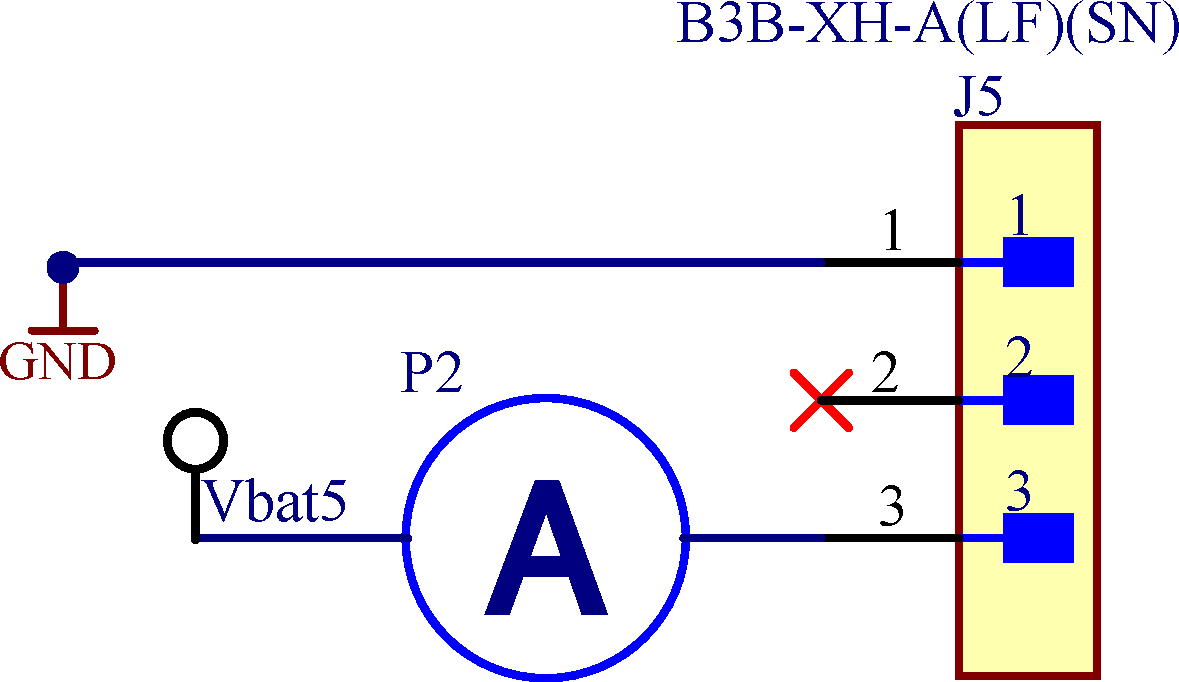
\includegraphics[width=.35\linewidth]{../figures/mesures/schema-courant}
	\caption{Schéma de mesure, courant}
	\label{fig:schema-courant}
	\source{Auteur}
\end{figure}

\subsubsection{Mesures}

\begin{table}[!h]
	\centering
	\resizebox{.8\textwidth}{!}{%
		\begin{tabular}{|c|l|l|c|c|}
			\hline
			\multicolumn{1}{|l|}{Index} & Etat du système & Condition                      & Courant [mA] & Symbol      \\ \hline
			[1]                         & Eteint.         & Mode auto-enclenchement OFF.   & 0.02         & $I_{off}$   \\ \hline
			[2]                         & Veille.         & Est passé par l'état SHUTDOWN. & 4.4          & $I_{sleep}$ \\ \hline
			[3]                         & Veille brutale. & Pas passé par l'état SHUTDOWN. & 9.56         & $I_{ws}$    \\ \hline
			[4]                         & Initialisation. & -                              & 90           & $I_{init}$  \\ \hline
			[5]                         & Logging.        & -                              & 100          & $I_{log}$   \\ \hline
			[6]                         & Shutdown.       & -                              & 83           & $I_{sh}$    \\ \hline
			[7]                         & Communication.  & USB branché.                   & 0            & $I_{usb}$   \\ \hline
		\end{tabular}%
	}
	\caption{Mesure des consommations}
	\label{tab:mes-cons}
	\source{Auteur}
\end{table}

Nous pouvons par les mesure de la table \ref{tab:mes-cons} déduire les éléments suivants : 

Où : 

Capacité de la batterie $C = 1600\;mAh$

\begin{tabular}{llll}
	$\bullet$ & Temps de logging &  (Table \ref{tab:mes-cons}-[5]) : & $T_l = \frac{C}{I_{log}} = 16h$. \\
	$\bullet$ & Temps épuisement batterie en veille & (Table \ref{tab:mes-cons}-[2]) : & $T_l = \frac{C}{I_{sleep}} = 364h = 15J$. \\
	$\bullet$ & Temps épuisement en veille brutale & (Table \ref{tab:mes-cons}-[3]) : & $T_l = \frac{C}{I_{ws}} = 167h = 7J$. \\
\end{tabular}

Par conséquent, les caractéristiques d'autonomie de la batterie sont suffisantes pour notre application. 

\subsection{Bus de communications}
Avec le code implémenté dans le microcontrôleur les différents périphèriques fonctionnement et la communication avec les différents bus sont fonctionnels, c'est pourquoi lors de cet section l'objectif principal est de  

\subsubsection{Communication I2C} \label{ssec:Comm-I2C}
\paragraph{Méthode de mesure}
\paragraph{Mesures}

\subsubsection{Communication UART} \label{ssec:Comm-UART}
\paragraph{Méthode de mesure}
\paragraph{Mesures}

\subsubsection{Communication SPI, carte SD} \label{ssec:Comm-SPI}
\paragraph{Méthode de mesure}
\paragraph{Mesures}

\section{Caractéristiques du produit fini} \label{sec:Carac-finis}